\documentclass[tikz,border=7pt]{standalone}
\usepackage{amsmath,amssymb}
\usetikzlibrary{arrows.meta,positioning,calc}
\begin{document}
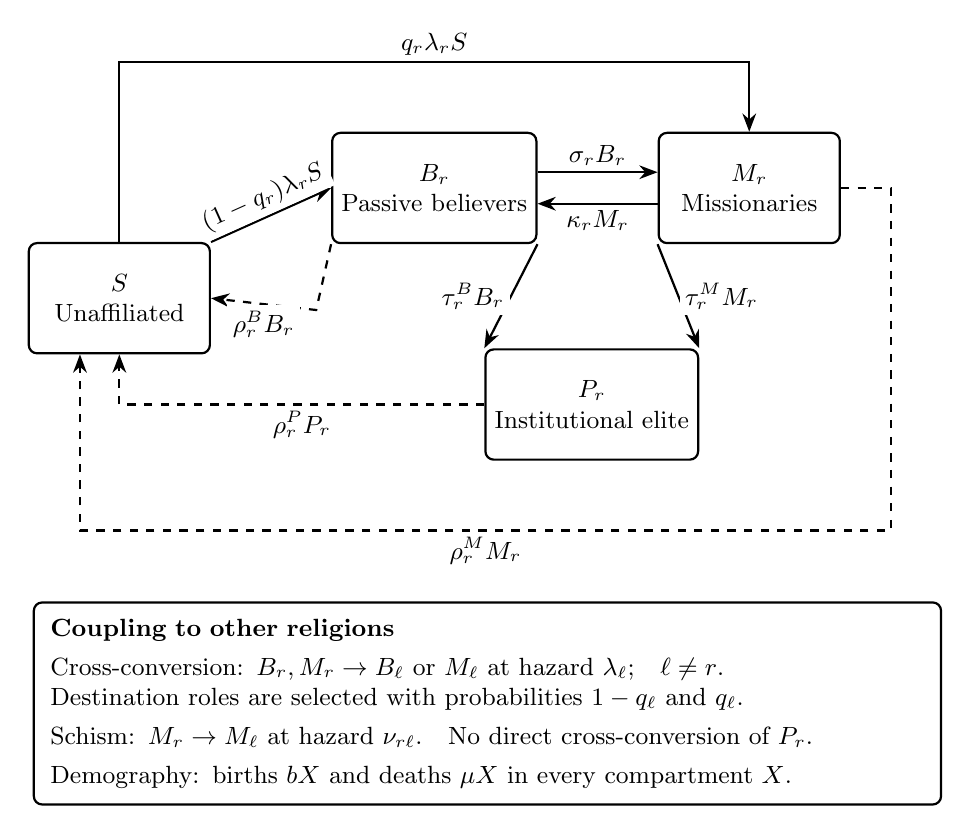
\begin{tikzpicture}[>=Stealth,thick, every node/.style={font=\small},
state/.style={draw,rounded corners=3pt,minimum width=23mm,minimum height=14mm,align=center},
lab/.style={fill=white,inner sep=2pt,font=\small}]
\node[state] (s) at (0,1.2) {$S$\\Unaffiliated};
\node[state] (b) at (4,2.6) {$B_r$\\Passive believers};
\node[state] (m) at (8,2.6) {$M_r$\\Missionaries};
\node[state] (p) at (6,-.15) {$P_r$\\Institutional elite};
\draw[->] (s.north east) -- node[lab,above,sloped] {$(1-q_r)\lambda_r S$} (b.west);
\draw[->] (s.north) -- (0,4.2) -- node[lab,above] {$q_r\lambda_r S$} (8,4.2) -- (m.north);
\draw[->] ([yshift=2mm]b.east) -- node[lab,above] {$\sigma_r B_r$} ([yshift=2mm]m.west);
\draw[->] ([yshift=-2mm]m.west) -- node[lab,below] {$\kappa_r M_r$} ([yshift=-2mm]b.east);
\draw[->] (b.south east) -- node[lab,left] {$\tau_r^B B_r$} (p.north west);
\draw[->] (m.south west) -- node[lab,right] {$\tau_r^M M_r$} (p.north east);
\draw[->,dashed] (b.south west) -- (2.5,1.05) -- node[lab,below] {$\rho_r^B B_r$} (s.east);
\draw[->,dashed] (m.east) -- (9.8,2.6) -- (9.8,-1.75) -- node[lab,below] {$\rho_r^M M_r$} (-.5,-1.75) -- ([xshift=-5mm]s.south);
\draw[->,dashed] (p.west) -- node[lab,below] {$\rho_r^P P_r$} (0,-.15) -- (s.south);
\node[draw,rounded corners=3pt,align=left,anchor=north west,inner sep=6pt,text width=11.1cm] at (-1.1,-2.65) {
\textbf{Coupling to other religions}\\[3pt]
Cross-conversion: $B_r,M_r\to B_\ell$ or $M_\ell$ at hazard $\lambda_\ell$;\quad $\ell\ne r$.\\
Destination roles are selected with probabilities $1-q_\ell$ and $q_\ell$.\\[3pt]
Schism: $M_r\to M_\ell$ at hazard $\nu_{r\ell}$.\quad No direct cross-conversion of $P_r$.\\[3pt]
Demography: births $bX$ and deaths $\mu X$ in every compartment $X$.};
\end{tikzpicture}
\end{document}
